\documentclass[tikz,border=9pt]{standalone}
\usepackage[T1]{fontenc}
\usepackage{lmodern}
\usepackage{amsmath,amssymb}
\usetikzlibrary{arrows.meta,positioning}
\definecolor{ink}{HTML}{203044}
\definecolor{line}{HTML}{798899}
\definecolor{low}{HTML}{EAF1F8}
\definecolor{high}{HTML}{B9CDE1}
\definecolor{panel}{HTML}{F4F6F8}
\begin{document}
\pagecolor{white}
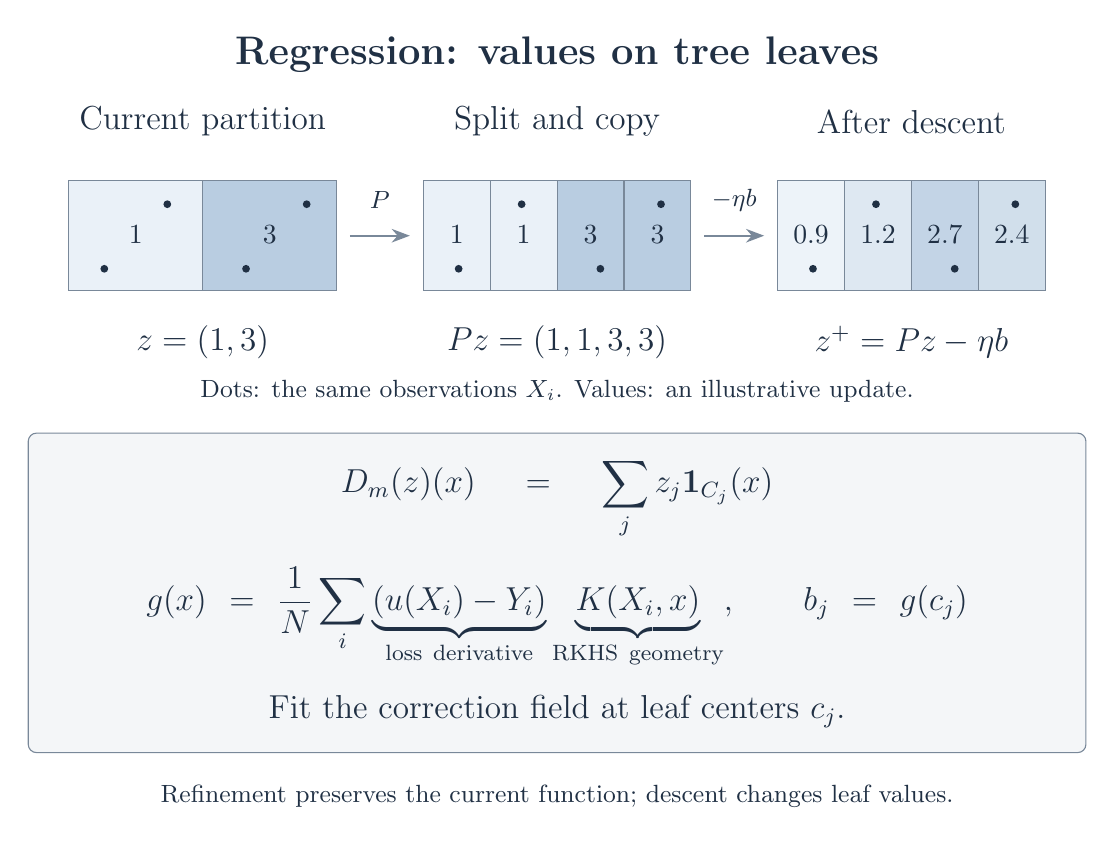
\begin{tikzpicture}[
  text=ink,
  arrow/.style={-{Stealth[length=2.3mm]},draw=line,line width=.8pt},
  label/.style={font=\large,align=center},
  box/.style={draw=line,rounded corners=3pt,fill=panel,
    text width=12.8cm,align=center,inner sep=9pt,font=\large}
]
  \node[font=\Large\bfseries] at (4.5,3.0)
    {Regression: values on tree leaves};
  \node[label] at (0,2.15) {Current partition};
  \node[label] at (4.5,2.15) {Split and copy};
  \node[label] at (9,2.15) {After descent};

  \fill[low] (-1.7,0) rectangle (0,1.4);
  \fill[high] (0,0) rectangle (1.7,1.4);
  \draw[draw=line] (-1.7,0) rectangle (1.7,1.4);
  \draw[draw=line] (0,0) -- (0,1.4);
  \node at (-.85,.72) {\(1\)};
  \node at (.85,.72) {\(3\)};

  \fill[low] (2.8,0) rectangle (4.5,1.4);
  \fill[high] (4.5,0) rectangle (6.2,1.4);
  \draw[draw=line] (2.8,0) rectangle (6.2,1.4);
  \foreach \x in {3.65,4.5,5.35}
    \draw[draw=line] (\x,0) -- (\x,1.4);
  \foreach \x/\v in {3.225/1,4.075/1,4.925/3,5.775/3}
    \node at (\x,.72) {\(\v\)};

  \fill[low!85!white] (7.3,0) rectangle (8.15,1.4);
  \fill[low!75!high] (8.15,0) rectangle (9,1.4);
  \fill[high!85!white] (9,0) rectangle (9.85,1.4);
  \fill[high!65!white] (9.85,0) rectangle (10.7,1.4);
  \draw[draw=line] (7.3,0) rectangle (10.7,1.4);
  \foreach \x in {8.15,9,9.85}
    \draw[draw=line] (\x,0) -- (\x,1.4);
  \foreach \x/\v in {7.725/0.9,8.575/1.2,9.425/2.7,10.275/2.4}
    \node at (\x,.72) {\(\v\)};

  \foreach \shift in {0,4.5,9}{
    \foreach \x/\y in {-1.25/.28,-.45/1.1,.55/.28,1.32/1.1}
      \fill[ink] ({\shift+\x},\y) circle (1.4pt);
  }
  \draw[arrow] (1.87,.7) -- (2.63,.7);
  \draw[arrow] (6.37,.7) -- (7.13,.7);
  \node[label,font=\small] at (2.25,1.15) {\(P\)};
  \node[label,font=\small] at (6.75,1.15) {\(-\eta b\)};

  \node[label] at (0,-.65) {\(z=(1,3)\)};
  \node[label] at (4.5,-.65) {\(Pz=(1,1,3,3)\)};
  \node[label] at (9,-.65) {\(z^+=Pz-\eta b\)};
  \node[font=\small,align=center] at (4.5,-1.28)
    {Dots: the same observations \(X_i\). Values: an illustrative update.};

  \node[box,anchor=north] (summary) at (4.5,-1.8) {
    \(\displaystyle D_m(z)(x)=\sum_j z_j\mathbf 1_{C_j}(x)\)
    \\[9pt]
    \(\displaystyle g(x)=\frac1N\sum_i
      \underbrace{(u(X_i)-Y_i)}_{\text{loss derivative}}
      \underbrace{K(X_i,x)}_{\text{RKHS geometry}},
      \qquad b_j=g(c_j)\)
    \\[9pt]
    Fit the correction field at leaf centers \(c_j\).
  };
  \node[label,font=\small,below=8pt of summary]
    {Refinement preserves the current function; descent changes leaf values.};
\end{tikzpicture}
\end{document}
